\chapter{วิธีการดำเนินการวิจัย}
\label{chapter:experiment}

\section{วิเคราะห์ความต้องการ}
\subsection{ความต้องการส่วนหน้าที่หลักของระบบ (Functional Requirement)}
\begin{itemize}
    \itemsep0em
    \item หุ่นยนต์สามารถทำตามชุดคำสั่งจากแผ่นคำสั่งได้
    \item หุ่นยนต์สามารถอ่าน QR Code บนแผ่นคำสั่งได้
\end{itemize}

\subsection{ความต้องการส่วนที่ไม่ใช่หน้าที่หลักของระบบ (Non-functional Requirement)}
\begin{itemize}
    \itemsep0em
    \item ออกแบบอุปกรณ์ให้มีความปลอดภัยต่อการใช้งานของเด็ก
    \item หุ่นยนต์สามารถอ่านข้อมูลจากแผ่นคำสั่งได้ถูกต้อง
    \item ใช้งานง่าย
    \item รองรับการขยายตัวของระบบ
\end{itemize}

\section{การวิเคราะห์และออกแบบระบบ}
\subsection{การออกแบบอุปกรณ์}
สื่อการเรียนรู้การคิดเชิงคำนวณในรูปแบบการเขียนโปรแกรมแบบจับต้องได้พัฒนาขึ้นเพื่อเพิ่มประสิทธิภาพ และสนับสนุนการเรียนรู้ทักษะการคิดเชิงคำนวณแก่เด็ก และเยาวชน ประกอบด้วย 3 ส่วนหลัก คือ หุ่นยนต์เคลื่อนที่ได้ แผ่นคำสั่ง และแผนที่แบบตาราง 

ในส่วนของวัสดุและอุปกรณ์สำหรับทำตัวหุ่นยนต์จะมีความปลอดภัยและมีรูปลักษณ์ที่เหมาะสำหรับการใช้งานของเด็ก เพิ่มความปลอดภัยด้วยการใช้วัสดุที่เป็น Food Grade และรูปทรงที่ไม่เป็นอันตรายต่อการใช้งานด้วยการออกแบบให้มีส่วนโค้งเพื่อลดความแหลมคม
\begin{figure}[ht]
    \centering
    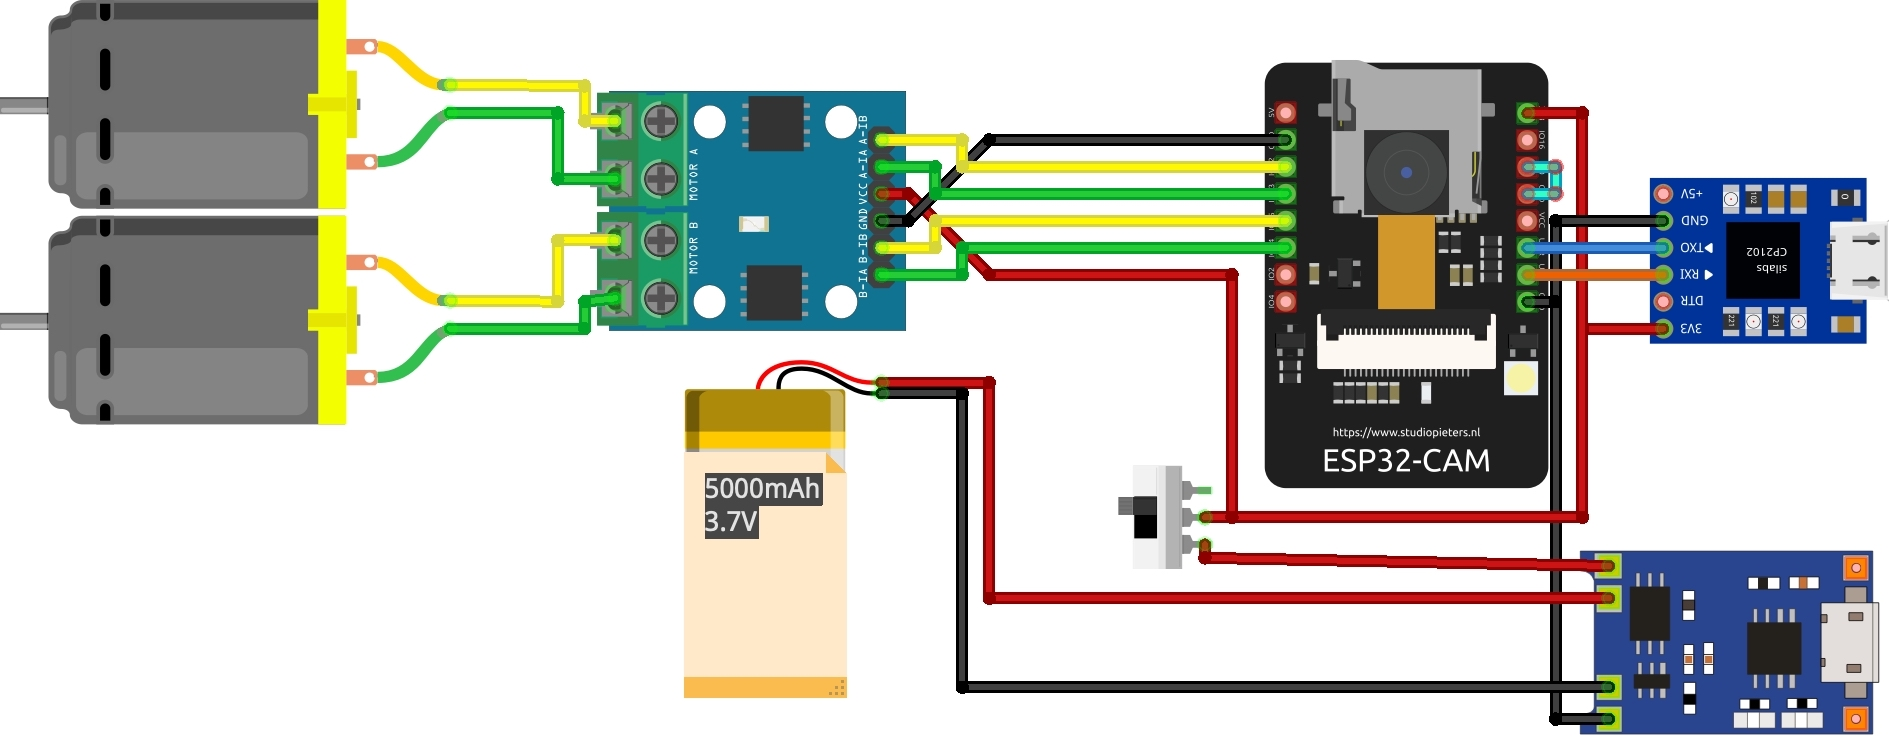
\includegraphics[width=120mm,scale=0.6]{circuit _sketch.jpg}
    \caption{การออกแบบวงจร}
    \label{fig:circuit}
\end{figure}

\begin{figure}[ht]
    \centering
    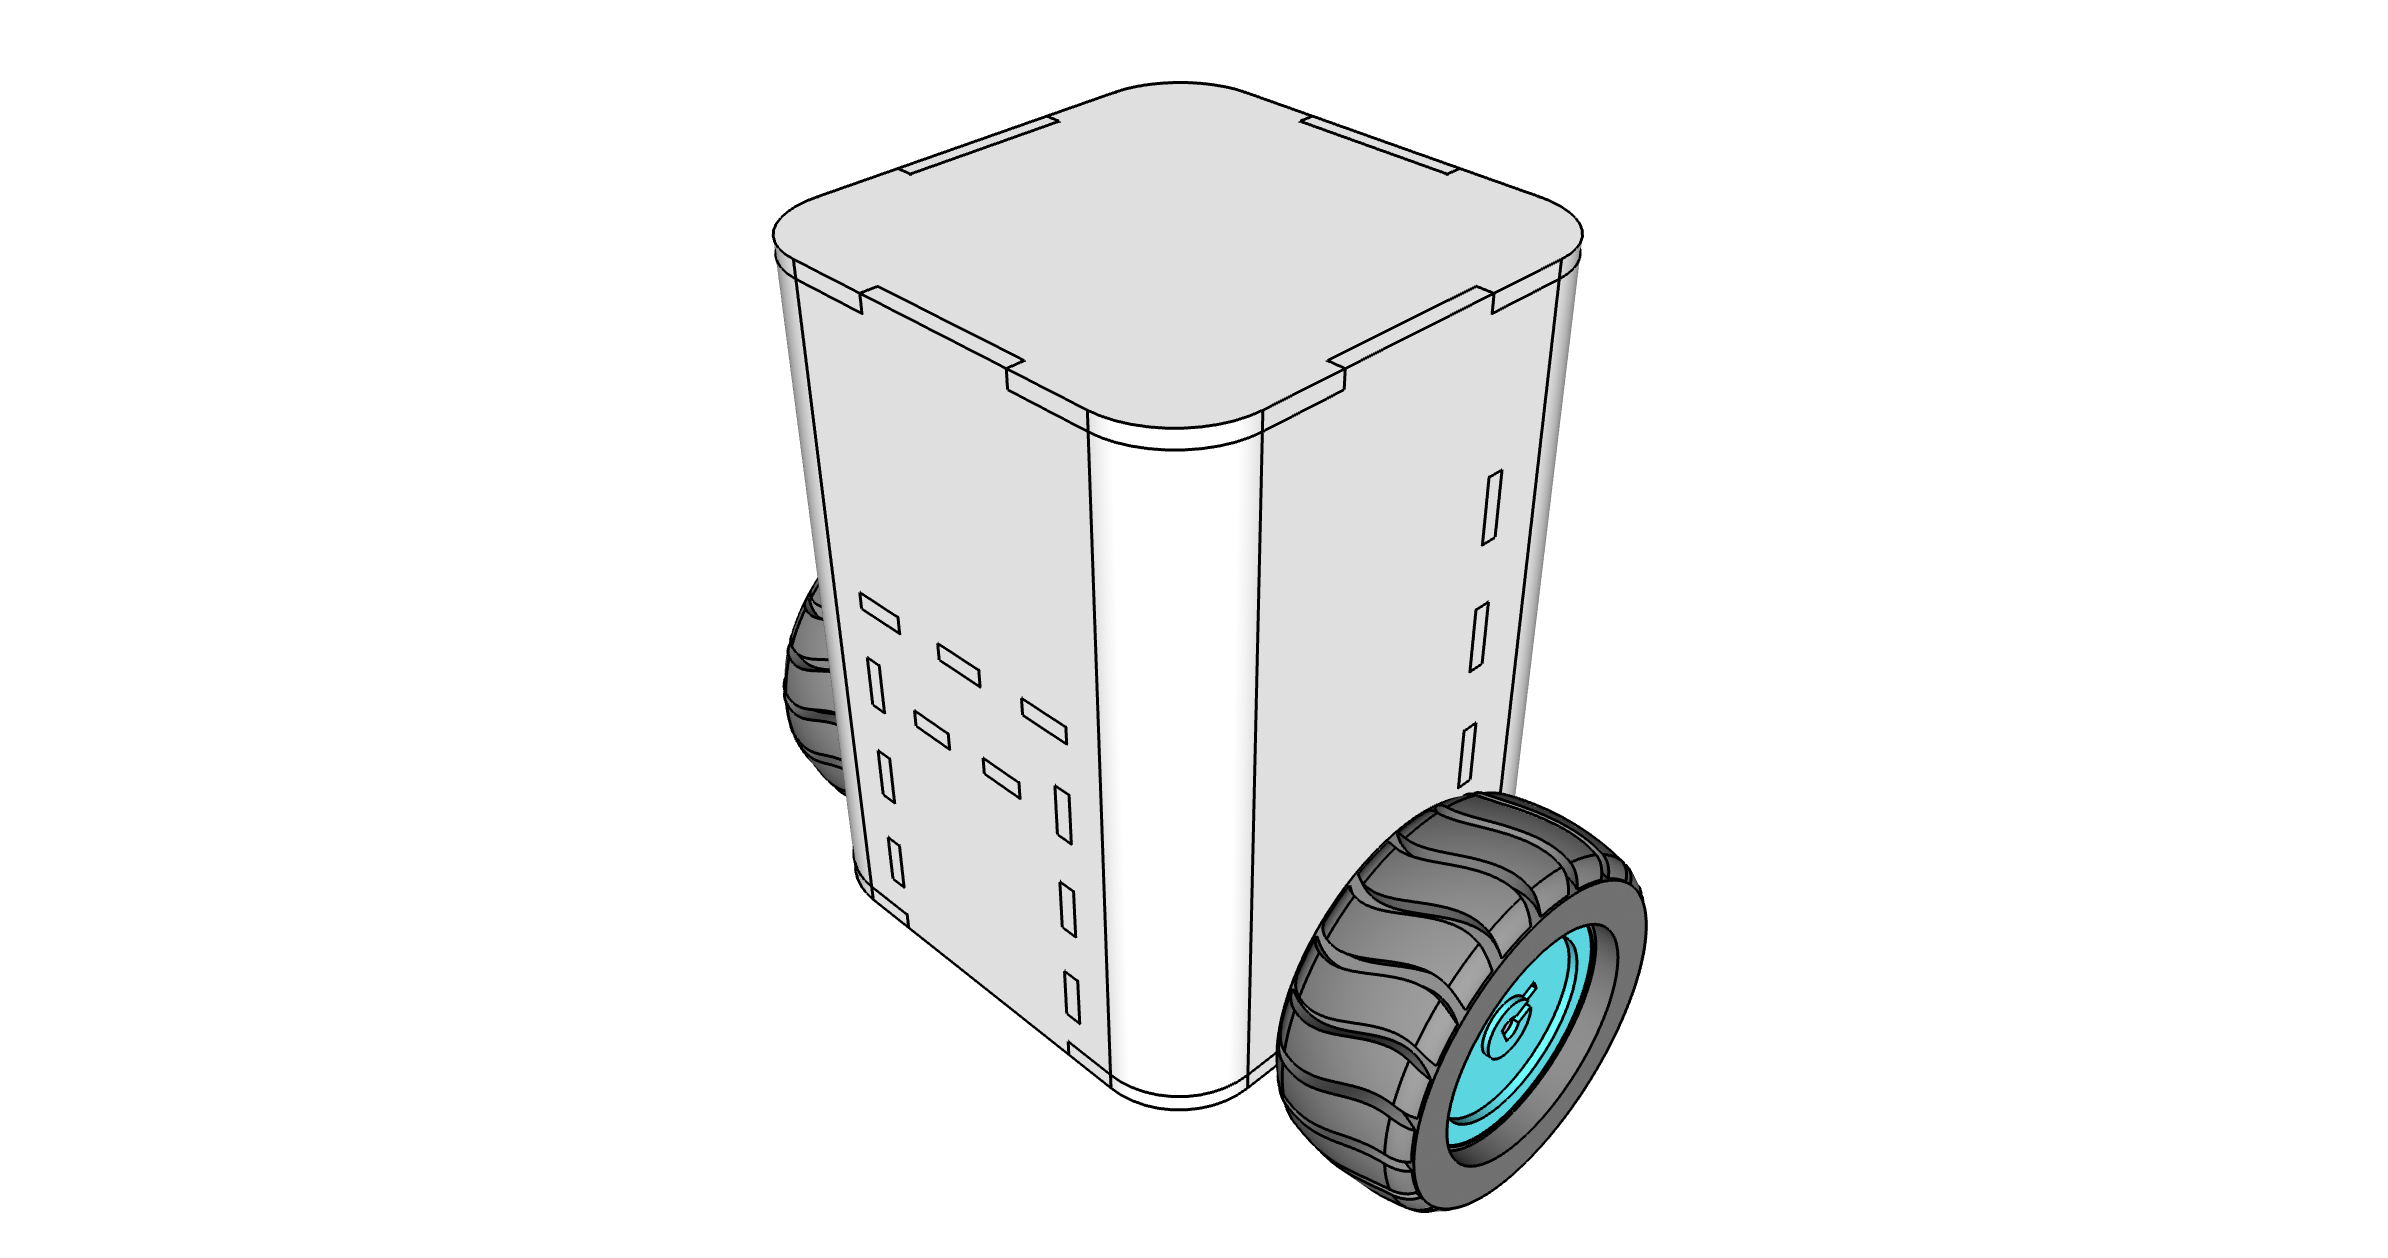
\includegraphics[width=120mm,scale=0.6]{model1.PNG}
    \caption{การออกแบบหุ่นยนต์}
    \label{fig:circuit}
\end{figure}

\subsection{แผนภาพยูสเคส (Use Case Diagram)}
\begin{figure}[ht]
    \centering
    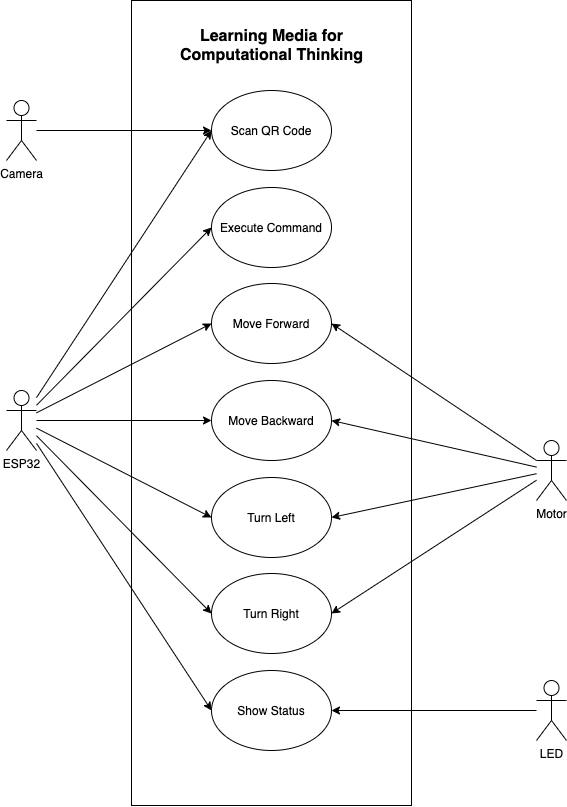
\includegraphics[width=120mm,scale=0.6]{Use_Case_Diagram.png}
    \caption{Use case diagram}
    \label{fig:Use_Case_Diagram}
\end{figure}
